%%%%%%%%%%%%%%%%%%%%%%%%%%%%%%%%%%%%%%%%%%%%%%%%%%%%%%%%%%
%%%%%%%%%%%%%%%%%%%%%%%%%%%%%%%%%%%%%%%%%%%%%%%%%%%%%%%%%%
%%          Written by Nicolas Bigaouette               %%
%%                    Winter 2008                       %%
%%              nbigaouette@gmail.com                   %%
%%%%%%%%%%%%%%%%%%%%%%%%%%%%%%%%%%%%%%%%%%%%%%%%%%%%%%%%%%
%%%%%%%%%%%%%%%%%%%%%%%%%%%%%%%%%%%%%%%%%%%%%%%%%%%%%%%%%%

\newcommand{\TITLE}{Change to Document's Title}
\newcommand{\AUTHOR}{Change to Document's Author}

\documentclass[12pt,letterpaper]{article}
% \documentclass[12pt,letterpaper,draft]{article}
\title{\TITLE}
\date{}
\author{\AUTHOR}

%%%%%%%%%%%%%%%%%%%%%%%%%%%%%%%%%%%%%%%%%%%%%%%%%%%%%%%
% Useful macros
%%%%%%%%%%%%%%%%%%%%%%%%%%%%%%%%%%%%%%%%%%%%%%%%%%%%%%%%%%%%%%%%%%%%%%%%%%%%%%%%%%%%%%
%%%%%%%%%%%%%%%%%%%%%%%%%%%%%%%%%%%%%%%%%%%%%%%%%%%%%%%%%%%%%%%%%%%%%%%%%%%%%%%%%%%%%%
%%                             Usefull macros                                       %%
%%                           Nicolas Bigaouette                                     %%
%%                          nbigaouette@gmail.com                                   %%
%%%%%%%%%%%%%%%%%%%%%%%%%%%%%%%%%%%%%%%%%%%%%%%%%%%%%%%%%%%%%%%%%%%%%%%%%%%%%%%%%%%%%%
%%%%%%%%%%%%%%%%%%%%%%%%%%%%%%%%%%%%%%%%%%%%%%%%%%%%%%%%%%%%%%%%%%%%%%%%%%%%%%%%%%%%%%

% \newcommand{\vecnabla}{\vec{\nabla}}
\newcommand{\vecnabla}{\bm{\nabla}}
\newcommand{\laplacien}[1]{\vecnabla^2 #1}           % Laplacien
\newcommand{\laplacient}[1]{\vecnabla_{\bot}^{2} #1} % Laplacien transverse
\newcommand{\gradient}[1]{\vecnabla #1}              % Gradient
\newcommand{\grad}[1]{\vecnabla #1}                  % Gradient
\newcommand{\divergence}[1]{\vecnabla \cdot #1}      % Divergence
\newcommand{\rotationnel}[1]{\vecnabla \times #1}    % Rotationnel

\newcommand{\mum}{\mu \textrm{m}}                               % mu m

\newcommand{\del}{\partial}                                     % del

\newcommand{\delx}[1]{\frac{\del #1}{\del x}}                   % del ? / delx
\newcommand{\dely}[1]{\frac{\del #1}{\del y}}                   % del ? / dely
\newcommand{\delz}[1]{\frac{\del #1}{\del z}}                   % del ? / delz
\newcommand{\delr}[1]{\frac{\del #1}{\del r}}                   % del ? / delr
\newcommand{\delt}[1]{\frac{\del #1}{\del t}}                   % del ? / delt
\newcommand{\deli}[2]{\frac{\del #1}{\del #2}}                  % del ? / del?

\newcommand{\delxs}[1]{\frac{\del^2 #1}{\del x^2}}              % del^2 ? / delx^2
\newcommand{\delys}[1]{\frac{\del^2 #1}{\del y^2}}              % del^2 ? / dely^2
\newcommand{\delzs}[1]{\frac{\del^2 #1}{\del z^2}}              % del^2 ? / delz^2
\newcommand{\delts}[1]{\frac{\del^2 #1}{\del t^2}}              % del^2 ? / delt^2
\newcommand{\delis}[2]{\frac{\del^2 #1}{\del #2^2}}             % del^2 ? / del?^2

\newcommand{\dx}[1]{\frac{\textrm{d} #1}{\textrm{d} x}}         % d ? / dx
\newcommand{\dy}[1]{\frac{\textrm{d} #1}{\textrm{d} y}}         % d ? / dy
\newcommand{\dz}[1]{\frac{\textrm{d} #1}{\textrm{d} z}}         % d ? / dz
\newcommand{\di}[2]{\frac{\textrm{d} #1}{\textrm{d} #2}}        % d ? / d?

\newcommand{\dxs}[1]{\frac{\textrm{d}^2 #1}{\textrm{d}x^2}}     % d^2 ? / dx^2
\newcommand{\dys}[1]{\frac{\textrm{d}^2 #1}{\textrm{d}y^2}}     % d^2 ? / dy^2
\newcommand{\dzs}[1]{\frac{\textrm{d}^2 #1}{\textrm{d}z^2}}     % d^2 ? / dz^2
\newcommand{\dis}[2]{\frac{\textrm{d}^2 #1}{\textrm{d}#2^2}}    % d^2 ? / d?^2

\newcommand{\dtreal}[1]{\frac{\textrm{d} #1}{\textrm{d} t}}         % d ? / dt
\newcommand{\dtsreal}[1]{\frac{\textrm{d}^2 #1}{\textrm{d}t^2}}     % d^2 ? / dt^2
\newcommand{\dt}[1]{\dot{#1}}                                   % d ? / dt
\newcommand{\dts}[1]{\ddot{#1}}                                 % d^2 ? / dt^2

\newcommand{\erf}[1]{~\textrm{erf} \left\{#1\right\}}                      % erf{?}
\newcommand{\ex}[1]{\exp{ \left\{ #1 \right\}}}                 % exp{?}
\newcommand{\ep}[1]{\textrm{e}^{\left( #1 \right) }}            % e^(?)
\newcommand{\e}[1]{\textrm{e}^{#1}}                             % e^?
\newcommand{\lnp}[1]{\textrm{ln} \left( #1 \right)}            % ln(?)
\newcommand{\logp}[1]{\textrm{log} \left( #1 \right)}          % log(?)
\newcommand{\cosinus}[1]{\cos #1 }                % cos()
% \newcommand{\cosinus}[1]{\cos \left( #1 \right)}                % cos()
\newcommand{\cosp}[1]{\cos \left( #1 \right)}                % cos()
\newcommand{\cosine}[1]{\cosinus{#1}}                           % cos()
\newcommand{\sinus}[1]{\sin #1 }                  % sin()
\newcommand{\sinp}[1]{\sin \left( #1 \right)}                  % sin()
% \newcommand{\sinus}[1]{\sin \left( #1 \right)}                  % sin()
\newcommand{\sine}[1]{\sinus{#1}}                               % sin()
\newcommand{\sinec}[1]{\textrm{ sinc} \left( #1 \right)}        % sinc()
\newcommand{\sinecsquared}[1]{\textrm{ sinc}^2 \left( #1 \right)} % sinc^2()
\newcommand{\cossquared}[1]{\cos^2 #1 }           % cos^2()
\newcommand{\sinsquared}[1]{\sin^2 #1 }           % sin^2()
% \newcommand{\cossquared}[1]{\cos^2 \left( #1 \right)}           % cos^2()
% \newcommand{\sinsquared}[1]{\sin^2 \left( #1 \right)}           % sin^2()
\newcommand{\cosinesquared}[1]{\cossquared{#1}}                 % cos^2()
\newcommand{\sinesquared}[1]{\sinsquared{#1}}                   % sin^2()
\newcommand{\acos}[1]{\textrm{acos} \left( #1 \right)}          % acos()
\newcommand{\asin}[1]{\textrm{asin} \left( #1 \right)}          % asin()
\newcommand{\atan}[1]{\textrm{atan} \left( #1 \right)}          % atan()
\newcommand{\sech}[1]{\textrm{sech} \left( #1 \right)}          % sech()
\newcommand{\tanhyp}[1]{\textrm{tanh} \left( #1 \right)}          % tanh()
\newcommand{\sechsquared}[1]{\textrm{sech}^2 \left( #1 \right)} % sech^2()

\newcommand{\dix}[1]{\times 10^{#1}}                            % ? x 10^?

\newcommand{\epsz}{\epsilon_0}
\newcommand{\epsr}{\epsilon_r}
\newcommand{\muz}{\mu_0}
\newcommand{\om}{\omega}
\newcommand{\omi}[1]{\omega_{#1}}
\newcommand{\omegaz}{\omega_0}
\newcommand{\omegasquared}{\omega^2}
\newcommand{\omegazsquared}{\omega_0^2}
\newcommand{\omegazsquaredomegasquared}{\omegazsquared - \omegasquared}

% \newcommand{\ve}[1]{\vec{#1}}
\newcommand{\ve}[1]{\textbf{#1}}
\newcommand{\vE}{\ve{E}}
\newcommand{\vA}{\ve{A}}
\newcommand{\vB}{\ve{B}}
\newcommand{\vF}{\ve{F}}
\newcommand{\vP}{\ve{P}}
\newcommand{\vS}{\ve{S}}
\newcommand{\va}{\ve{a}}
\newcommand{\vb}{\ve{b}}
\newcommand{\vc}{\ve{c}}
\newcommand{\vd}{\ve{d}}
\renewcommand{\vee}{\ve{e}}
\newcommand{\vf}{\ve{f}}
\newcommand{\vg}{\ve{g}}
\newcommand{\vh}{\ve{h}}
\newcommand{\vi}{\ve{i}}
\newcommand{\vj}{\ve{j}}
\newcommand{\vk}{\ve{k}}
\newcommand{\vl}{\ve{l}}
\newcommand{\vm}{\ve{m}}
\newcommand{\vp}{\ve{p}}
\newcommand{\vq}{\ve{q}}
\newcommand{\vr}{\ve{r}}
\newcommand{\vqd}{\dot{\vq}}
\newcommand{\vv}{\ve{v}}
\newcommand{\vt}{\ve{t}}
\newcommand{\vx}{\ve{x}}
\newcommand{\vz}{\ve{z}}

\newcommand{\vmu}{\bm{\mu}}
\newcommand{\vDelta}{\bm{\Delta}}

\newcommand{\hvp}{\hat{\textbf{p}}}
\newcommand{\hvq}{\hat{\textbf{q}}}
\newcommand{\hvr}{\hat{\textbf{r}}}
\newcommand{\hvu}{\hat{\textbf{u}}}
\newcommand{\hvx}{\hat{\textbf{x}}}
\newcommand{\hvy}{\hat{\textbf{y}}}
\newcommand{\hvz}{\hat{\textbf{z}}}
\newcommand{\hvtheta}{\hat{\bm{\theta}}}
\newcommand{\hvphi}{\hat{\bm{\phi}}}

\renewcommand{\t}[1]{\tilde{#1}}
\newcommand{\tE}{\t{E}}
\newcommand{\tP}{\t{P}}
\newcommand{\tvE}{\t{\vE}}
\newcommand{\tvP}{\t{\vP}}
\newcommand{\tA}{\tilde{\textrm{A}}}
\newcommand{\tvA}{\tilde{\vA}}

\newcommand{\vEo}{\vE_{\omega}}
\newcommand{\vEto}{\vE_{2 \omega}}
\newcommand{\vPo}{\vP_{\omega}}
\newcommand{\vPto}{\vP_{2 \omega}}

\newcommand{\schrodinger}{Schr\"odinger }

\newcommand{\ver}{\ve{r}}
\newcommand{\unite}[1]{\textrm{#1}}
% \newcommand{\unite}[1]{~\textrm{#1}}
% \newcommand{\unites}[1]{\textrm{#1}}
\newcommand{\se}{\hspace{3pt}}                          % Espace pour les équations
\newcommand{\su}{\hspace{3pt}}                          % Espace pour les unités

\newcommand{\pa}[1]{\left( #1 \right)}
\newcommand{\cro}[1]{\left[ #1 \right]}
\newcommand{\bra}[1]{\left\{ #1 \right\}}

\newcommand{\ft}[1]{\textrm{FT}\pa{#1}}
\newcommand{\fti}[1]{\textrm{FT}^{-1}\pa{#1}}

\newcommand{\chiun}{\chi^{(1)}}
\newcommand{\chideux}{\chi^{(2)}}
\newcommand{\chitrois}{\chi^{(3)}}

\newcommand{\abs}[1]{\left| #1 \right|}

%%%%%%%%%%%%%%%%%%%%%%%%%%%%%%%%%%%%%%%%%%%%%%%%%%%%%%%%%%%%%%%%%%%%%%%%%%%%%%%%%%%%
%%%%%%%%%%%%%%%%%%%%%%%%%%%%%%%%%%%%%%%%%%%%%%%%%%%%%%%%%%%%%%%%%%%%%%%%%%%%%%%%%%%%



%%%%%%%%%%%%%%%%%%%%%%%%%%%%%%%%%%%%%%%%%%%%%%%%%%%%%%%
% Optional packages
%%%%%%%%%%%%%%%%%%%%%%%%%%%%%%%%%%%%%%%%%%%%%%%%%%%%%%%
\usepackage{amsmath}    % Subequations
\usepackage{bm}         % bold Greek letters
\usepackage{subfigure}  % Multiple figures
\usepackage{ltugcomn}   % 1/2 symbol
\usepackage{multirow}   % Multiple rows
% \usepackage{dcolumn}    % Align table columns on decimal point
% \biboptions{compress} % \usepackage[compress]{natbib}
\usepackage{url}        % Inclure url in text
%%%%%%%%%%%%%%%%%%%%%%%%%%%%%%%%%%%%%%%%%%%%%%%%%%%%%%%

%%%%%%%%%%%%%%%%%%%%%%%%%%%%%%%%%%%%%%%%%%%%%%%%%%%%%%%
% This template required packages
% \usepackage{ifthen}     % For optional compilation
\usepackage{ifpdf}      % For dvi/pdf optional compilation
%%%%%%%%%%%%%%%%%%%%%%%%%%%%%%%%%%%%%%%%%%%%%%%%%%%%%%%



\ifpdf
    %%%%%%%%%%%%%%%%%%%%%%%%%%%%%%%%%%%%%%%%%%%%%%%%%%%%%%%
    % PDF compilation with "pdflatex"
    %%%%%%%%%%%%%%%%%%%%%%%%%%%%%%%%%%%%%%%%%%%%%%%%%%%%%%%
    \def\pdfshellescape{1}
    \pdfcompresslevel=9
    \usepackage[pdftex]{graphicx}
    %%%
    % PDF options
    % See http://barrault.free.fr/ressources/rapports/pdflatex/
    \usepackage[pdftex,
        bookmarks = true,           % Enable bookmarks
        bookmarksnumbered = true,   % Enable numbered bookmarks
        bookmarksopen = false,      % Bookmarks are hidden when opening document
        unicode = true,             % Unicode character support in bookmarks
        %pdfpagemode = UseOutlines, % Show outline when opening document
        pdfpagemode = UseNone,      % Hide outline when opening document
        pdfstartview = FitH,        % Fit page width when opening document
        colorlinks,                 % Hyperlinks are colored
        urlcolor=blue,              % URL set to blue
        citecolor=black,
        linkcolor=black,
        pdfauthor={\AUTHOR},        % Macro expanding to author name (see top)
        pdftitle={\TITLE},          % Macro expanding to title (see top)
        plainpages = false,pdfpagelabels % See https://en.wikibooks.org/wiki/LaTeX/Hyperlinks#Problems_with_Links_and_Pages
    ]{hyperref}
    \usepackage[all]{hypcap}        % Make sure the links point to top of figures, not captions.
                                    % http://en.wikibooks.org/wiki/LaTeX/Labels_and_Cross-referencing#Issues_with_links_to_tables_and_figures_handled_by_hyperref
\else
    %%%%%%%%%%%%%%%%%%%%%%%%%%%%%%%%%%%%%%%%%%%%%%%%%%%%%%%
    % DVI compilation with "latex"
    %%%%%%%%%%%%%%%%%%%%%%%%%%%%%%%%%%%%%%%%%%%%%%%%%%%%%%%
    \usepackage[dvips]{graphicx}
    \newcommand{\url}[1]{{\color{blue}#1}}
\fi

%%%%%%%%%%%%%%%%%%%%%%%%%%%%%%%%%%%%%%%%%%%%%%%%%%%%%%%

%%%%%%%%%%%%%%%%%%%%%%%%%%%%%%%%%%%%%%%%%%%%%%%%%%%%%%%%%%
% Page format: reduce default margins
%%%%%%%%%%%%%%%%%%%%%%%%%%%%%%%%%%%%%%%%%%%%%%%%%%%%%%%%%%
\textheight=21cm
\textwidth=17.0cm
\oddsidemargin=0cm
\evensidemargin=0cm
\topmargin=0cm
\headsep=20pt
\topskip=10pt
\large
%%%%%%%%%%%%%%%%%%%%%%%%%%%%%%%%%%%%%%%%%%%%%%%%%%%%%%%%%%


\begin{document}


\maketitle
\tableofcontents

\newpage

\section{Macros}

Here's a list of macros defined in macros.tex:

\subsection{Nabla}
\begin{subequations}
\begin{align}
\textrm{\textbackslash vecnabla}            & = \vecnabla           \label{eqn:vnabla}      \\
\textrm{\textbackslash laplacien\{A\}}      & = \laplacien{A}       \label{eqn:laplacien}   \\
\textrm{\textbackslash laplacient\{A\}}     & = \laplacient{A}      \label{eqn:laplacient}  \\
\textrm{\textbackslash gradient\{A\}}       & = \gradient{A}        \label{eqn:gradient}    \\
\textrm{\textbackslash grad\{A\}}           & = \grad{A}            \label{eqn:grad}        \\
\textrm{\textbackslash divergence\{vB\}}    & = \divergence{\vB}    \label{eqn:divergence}  \\
\textrm{\textbackslash rotationnel\{vB\}}   & = \rotationnel{\vB}   \label{eqn:rotationnel}
\end{align}
\end{subequations}

\subsection{Units}
\begin{align}
\textrm{\textbackslash mum}                 & = \mum                \label{eqn:mum}
\end{align}


% \newpage
\section{Other useful information}

See also the \textit{The Not So Short Introduction to \LaTeXe}\cite{NotSoShort}
available online at \url{http://tobi.oetiker.ch/lshort/lshort.pdf} or
\url{http://www.ctan.org/tex-archive/info/lshort/english/lshort.pdf}.

\subsection{Example functions}
\begin{align}
F\pa{x} & = \int_{0}^{\infty} \frac{\sqrt{a + x}}{\pa{b + x}^5}~\textrm{d}x
\label{eqn:example}
\end{align}

\subsection{Citing}
When a label is attached to an equation, it can be cited. By adding ``\textbackslash label\{eqn:example\}'' in
the function's \textit{align} environment, it becomes possible to cite equation \eqref{eqn:example} with
``\textbackslash eqref\{eqn:example\}''.

To refence a book, article or other, use \BibTeX. Then cite the document
using its \BibTeX key with ``\textbackslash cite\{BibTeX key\}''. For example,
``\textbackslash cite\{Taflove2005\}'' will give the clickable link \cite{Taflove2005}
which points to the references section.



\subsection{Figures}
Figures should be in PDF or PNG format if compiling using \textbf{pdflatex} or EPS if compiling
with \textbf{latex} (resulting in a DVI file).

Since PDF is a vectorial format, figures in PDF will give higher quality results (if the figure
is in vectorial format that is). Figure \ref{fig:example_figure} shows an example.

\begin{figure}
\begin{center}
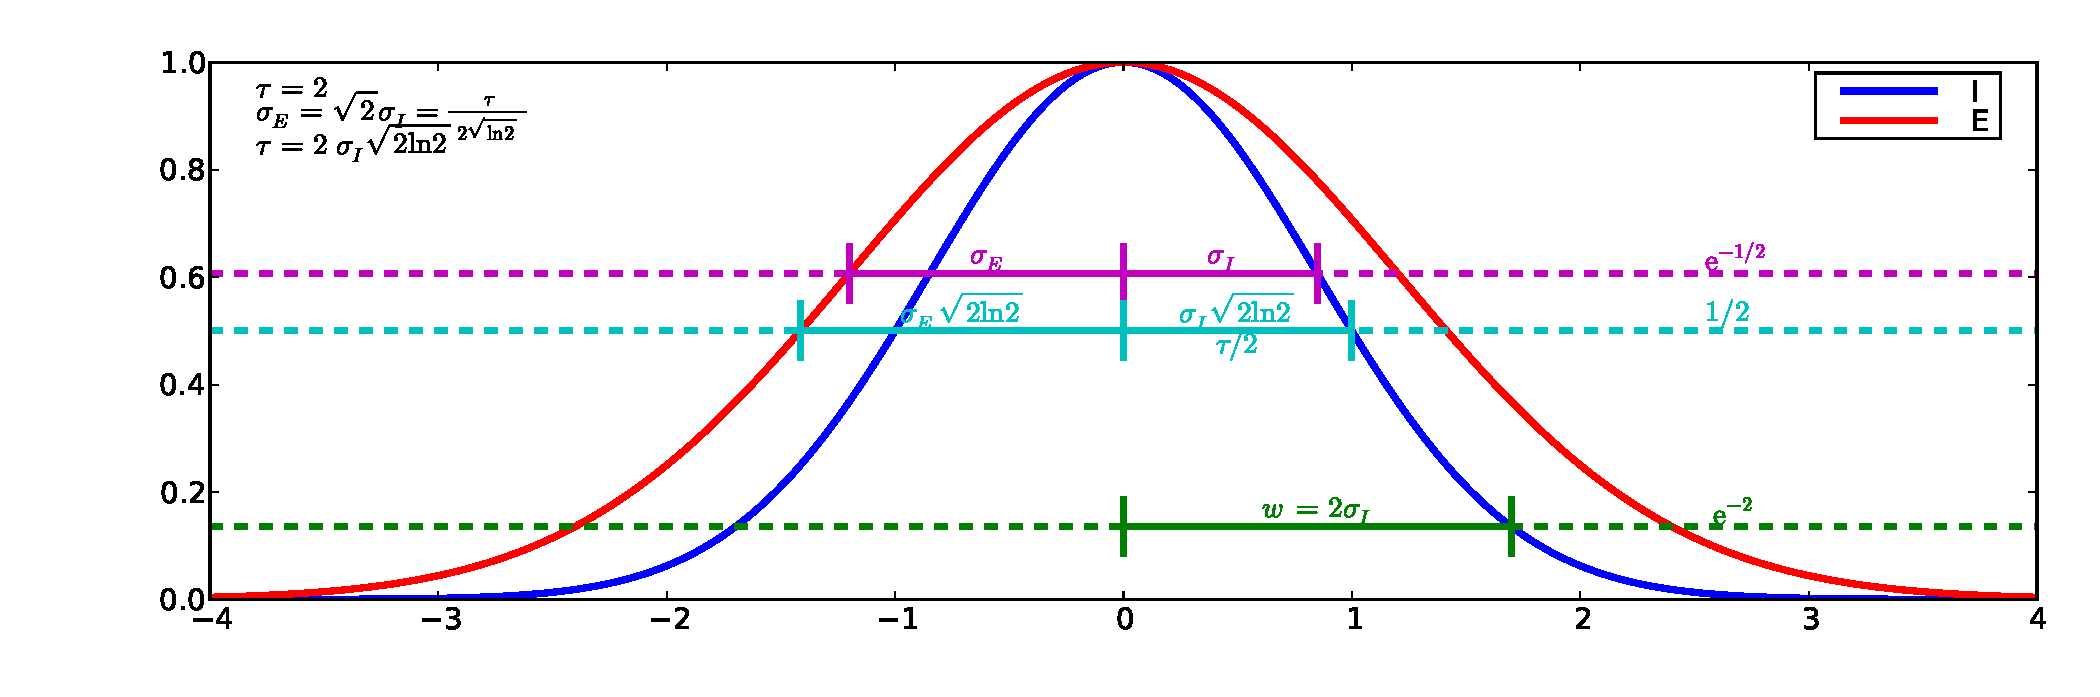
\includegraphics[width=\textwidth]{forme_I_E.pdf}
\end{center}
\caption{This is a caption}
\label{fig:example_figure}
\end{figure}


\subsection{Greek alphabet}

\begin{center}
\begin{tabular}{|l|c||l|c|l|c||l|c|} \hline
Code                        & Result            & Code                        & Result      & Code                        & Result          & Code                        & Result          \\ \hline \hline
\textbackslash alpha        & $\alpha$          & \textbackslash mu           & $\mu$       & \textbackslash chi          & $\chi$          & \textbackslash Sigma        & $\Sigma$        \\ \hline
\textbackslash beta         & $\beta$           & \textbackslash nu           & $\nu$       & \textbackslash psi          & $\psi$          & \textbackslash varSigma     & $\varSigma$     \\ \hline
\textbackslash gamma        & $\gamma$          & \textbackslash xi           & $\xi$       & \textbackslash omega        & $\omega$        & \textbackslash Upsilon      & $\Upsilon$      \\ \hline
\textbackslash delta        & $\delta$          & \textbackslash pi           & $\pi$       & \textbackslash Gamma        & $\Gamma$        & \textbackslash varUpsilon   & $\varUpsilon$   \\ \hline
\textbackslash epsilon      & $\epsilon$        & \textbackslash varpi        & $\varpi$    & \textbackslash varDelta     & $\varDelta$     & \textbackslash Phi          & $\Phi$          \\ \hline
\textbackslash varepsilon   & $\varepsilon$     & \textbackslash rho          & $\rho$      & \textbackslash Theta        & $\Theta$        & \textbackslash varPhi       & $\varPhi$       \\ \hline
\textbackslash zeta         & $\zeta$           & \textbackslash varrho       & $\varrho$   & \textbackslash varTheta     & $\varTheta$     & \textbackslash Psi          & $\Psi$          \\ \hline
\textbackslash eta          & $\eta$            & \textbackslash sigma        & $\sigma$    & \textbackslash Lambda       & $\Lambda$       & \textbackslash varPsi       & $\varPsi$       \\ \hline
\textbackslash theta        & $\theta$          & \textbackslash varsigma     & $\varsigma$ & \textbackslash varLambda    & $\varLambda$    & \textbackslash Omega        & $\Omega$        \\ \hline
\textbackslash vartheta     & $\vartheta$       & \textbackslash tau          & $\tau$      & \textbackslash Xi           & $\Xi$           & \textbackslash varOmega     & $\varOmega$     \\ \hline
\textbackslash iota         & $\iota$           & \textbackslash upsilon      & $\upsilon$  & \textbackslash varXi        & $\varXi$        &                             &                 \\ \hline
\textbackslash kappa        & $\kappa$          & \textbackslash phi          & $\phi$      & \textbackslash Pi           & $\Pi$           &                             &                 \\ \hline
\textbackslash lambda       & $\lambda$         & \textbackslash varphi       & $\varphi$   & \textbackslash varPi        & $\varPi$        &                             &                 \\ \hline
\end{tabular}
\end{center}



% \hypertarget{section:references}{}
% \nocite{*}
% \bibliography{references}
% % \bibliographystyle{model1-num-names}
% \bibliographystyle{plain}



\end{document}
